% Have someone read this chapter
% Add citations
  % Wu experiment (parity violation)
  %Super Kamiokande, MINOS
  %No$\nu$a, MACRO 
  %SNO,Gallex,
  %SAGE,  KamLAND 
  % DAYA  Bay,   RENO
% Red stuff!

\chapter{The theoretical framework}

\section{The Standard Model}
The Standard Model (SM) of particle physics is the most accurate theoretical description of the subatomic world and, in general, one of the most precisely tested theories in the history of physics.  The SM describes the strong, electromagnetic and weak interactions among  elementary particles in the framework of quantum field theory, accounting for the unification of electromagnetic and weak interactions for energies above the  vacuum expectation value of the Higgs field. The SM does not describe gravity or general relativity.

The Standard Model is a gauge theory based on the local group of symmetry
\begin{equation}
G_{SM} = SU(3)_C  \otimes SU(2)_T \otimes U(1)_Y
\label{eq:SMGroup}
\end{equation}

where the subscripts indicate the conserved charges: the strong charge, or color C, the weak isospin T (or rather its third component T3) and the hypercharge Y. These quantities can be related to the electric charge Q through the Gell-Mann-Nishijima relation:
\begin{equation}
Q = \frac{Y}{2} + T_3.
\end{equation}

In the quantum field framework, the elementary particles correspond to the irreducible representations of the G$_{SM}$ symmetry group. In particular, the particles are divided in two categories, fermions and bosons, according to their spin-statistics. Described by the Fermi-Dirac statistics, fermions have half-integer spin and are sometimes called ``matter-particles". Bosons or ``force carriers" have integer spin, follow the Bose-Einstein statistics and mediate the interaction between fermions. The fundamental fermions and their quantum numbers are listed in Tab \ref{tab:SMParticles}.

\begin{table}[]
\centering
\begin{tabular}{|cccc|c|c|c|}\hline
Generation               & I                   & II                  & III                 & T                       & Y                   & Q                   \\\hline

\multirow{6}{*}{Leptons}                          &                     &                     &                     &                         &                     &                     \\
& $\begin{pmatrix}\ \nu_e\\ e \end{pmatrix}_L$ & $\begin{pmatrix}\ \nu_\mu\\ \mu \end{pmatrix}_L$ & $\begin{pmatrix}\ \nu_\tau\\ \tau \end{pmatrix}_L$ & $\begin{matrix}\ 1/2\\ -1/2 \end{matrix}$ & $\begin{matrix}\ -1\\ -1 \end{matrix}$ & $\begin{matrix}\ 0\\ -1 \end{matrix}$ \\
                         &                     &                     &                     &                         &                     &                     \\
                         & $e_R$         & $\mu_R$      & $\tau_R$                  & 0                      & -2                  & 1    \\
                         &                     &                     &                     &                         &                     &                     \\\hline
\multirow{7}{*}{Quarks} 
                         &                     &                     &                     &                         &                     &                     \\
& $\begin{pmatrix}\ u\\ d' \end{pmatrix}_L$ & $\begin{pmatrix}\ c\\ s' \end{pmatrix}_L$ & $\begin{pmatrix}\ t\\ b' \end{pmatrix}_L$ & $\begin{matrix}\ 1/2\\ -1/2 \end{matrix}$ & $\begin{matrix}\ 1/3\\ 1/3 \end{matrix}$ & $\begin{matrix}\ 2/3\\ -1/3 \end{matrix}$ \\
                         &                     &                     &                     &                         &                     &                     \\
& $\begin{matrix}\ u_R\\ d'_R \end{matrix}$ & $\begin{matrix}\ c_R\\ s'_R \end{matrix}$ & $\begin{matrix}\ t_R\\ b'_R \end{matrix}$ & $\begin{matrix}\ 0\\ 0 \end{matrix}$ & $\begin{matrix}\ 4/3\\ -2/3 \end{matrix}$ & $\begin{matrix}\ 2/3\\ -1/3 \end{matrix}$ \\
                         &                     &                     &                     &                         &                     &                    \\\hline
\end{tabular}
\caption{SM elementary fermions. The subscripts L and R indicate respectively the negative helicity (left-handed) and the positive helicity (right-handed).}
\label{tab:SMParticles}
\end{table}

Quarks can interact via all three the fundamental forces; they are triplets of SU(3)$_C$, that is they can exist in three different colors: C = R, G, B. If one chooses a base where $u$, $c$ and $t$ quarks are simultaneously eigenstates of both the strong and the weak interactions, the remaining eigenstates are usually written as $d$, $s$ and $b$ for the strong interaction and $d'$, $s'$ and $b'$ for the weak interaction, because the latter ones are the result of a Cabibbo rotation on the first ones.
Charged leptons interact via the weak and the electromagnetic forces, while neutrinos only interact via the weak force. 
The gauge group univocally determines the number of gauge bosons that carry the interaction; the gauge bosons correspond to the generators of the group: eight gluons (g) for the strong interaction, one photon ($\gamma$) and three bosons (W$^\pm$, Z$^0$) for the electroweak interaction.
A gauge theory by itself can not provide a description of massive particles, but it is experimentally well know that most of the elementary particles have non-zero masses. The introduction of massive fields in the Standard Model lagrangian would make the theory non-renormalizable, and - so far - mathematically impossible to handle. This problem is solved in the Standard Model by the introduction of a scalar iso-doublet $\Phi(x)$, the Higgs field, which gives mass to W$^\pm$ and Z$^0$ gauge bosons through the electroweak symmetry breaking and to the fermions through Yukawa coupling \cite{Higgs1964,Higgs19642}.  The discovery of the Higgs boson in 2012 by the LHC experiments \cite{201230,Aad2012} marked the ultimate confirmation  of a long history of Standard Model successful predictions.

\section{Neutrinos:  tiny cracks in the Standard Model}
\subsection{Neutrinos in the Standard Model}
Neutrino were introduced in the SM as left-handed massless Weyl spinors.
The Dirac equation of motion
\begin{equation}
(i\gamma^ \mu \partial_\mu - m) \psi = 0
\end{equation}
for a fermionic field 
\begin{equation}
 \psi =  \psi_L +  \psi_R
\end{equation}
is equivalent to the equaitons
\begin{equation}
i\gamma^ \mu \partial_\mu  \psi_L = m \psi_R
\label{eq:15}
\end{equation}
\begin{equation}
i\gamma^ \mu \partial_\mu  \psi_R = m \psi_L
\label{eq:16}
\end{equation}

for the chiral fields $\psi_R$ and $\psi_L$, whose evolution in space and time is coupled through the mass $m$.
If the fermion is massless, the chiral fields decouple and the fermion can be described by a single Weyl spinor with two independent components~\cite{Weyl:10.2307}. Pauli initially rejected the description of a physical particle through a single Weyl spinor because of its implication of parity violation. In fact, since the spatial inversion operator throws $\psi_R \leftrightarrow \psi_L$, parity is conserved only if the both the chiral components exist at the same time.  For the neutrino introduction in the SM, experiments came in help of the theoretical description.  The constraint of parity conservation weakened after Wu's experiment in 1957 \cite{PhysRev.105.1413}. Additionally,  there was no experimental indication for massive neutrinos nor evidence of interaction via the neutrino right-handed component.% neutrinos likely interacted only via the left-handed component. 

The symmetry group $SU(2)_T \otimes U(1)_Y$ is the only group relevant for neutrino interactions. The SM electroweak lagrangian is the most general renormalizable lagrangian invariant under the local symmetry group $SU(2)_T \otimes U(1)_Y$. The lagrangian couples the weak isotopic spin doublets and singlets described in \ref{tab:SMParticles} with the gauge bosons  $A^{\mu}_{a}$ ($a$ $=$ 1,2,3) and $B^{\mu}$, and Higgs doublet $\Phi(x)$:

\begin{eqnarray}
\lefteqn{\mathcal{L} = i\sum_{\alpha=e,\mu,\tau} \bar{L}'_{\alpha L}  \slashed D L'_{\alpha L} + 
 i\sum_{\alpha=1,2,3} \bar{Q}'_{\alpha L}  \slashed D Q'_{\alpha L} {}}
 \nonumber\\
 & & {} + i\sum_{\alpha=e,\mu,\tau} \bar{l}'_{\alpha R}  \slashed D l'_{\alpha R} + i\sum_{\alpha=d,s,b} \bar{q}'^D_{\alpha R}  \slashed D q'^D_{\alpha R} + i\sum_{\alpha=u,c,t} \bar{q}'^U_{\alpha R}  \slashed D q'^U_{\alpha R}
 \nonumber\\
 & & {} -\frac{1}{4}A_{\mu \nu}A^{\mu \nu} - \frac{1}{4}B_{\mu \nu}B^{\mu \nu}
 \nonumber\\
 & & {} +(D_{\rho}\Phi)^\dagger(D^{\rho}\Phi) - \mu^2\Phi^\dagger\Phi - \lambda(\Phi^\dagger\Phi)^2 
 \nonumber\\
 & & {} -\sum_{\alpha,\beta=e,\mu,\tau} \Big(Y'^l_{\alpha\beta}\bar{L}'_{\alpha L}  \Phi l'_{\beta R} + Y'^{l*}_{\alpha\beta}\bar{l}'_{\beta R}  \Phi^\dagger L'_{\alpha L}\Big)
  \nonumber\\
 & & {} -\sum_{\alpha=1,2,3} \sum_{\beta=d,s,b} \Big(Y'^D_{\alpha\beta}\bar{Q}'_{\alpha L}  \Phi q'^D_{\beta R} + Y'^{D*}_{\alpha\beta}\bar{q}'^D_{\beta R}  \Phi^\dagger Q'_{\alpha L}\Big)
  \nonumber\\
 & & {} -\sum_{\alpha=1,2,3} \sum_{\beta=u,c,t} \Big(Y'^U_{\alpha\beta}\bar{Q}'_{\alpha L}   \widetilde{\Phi} q'^U_{\beta R} + Y'^{U*}_{\alpha\beta}\bar{q}'^U_{\beta R} \widetilde{\Phi}^\dagger Q'_{\alpha L}\Big).
\end{eqnarray}

The first two lines of the lagrangian summarize the kinetic terms for the fermionic fields and their coupling to the gauge bosons $A^{\mu\nu}_a$, $B^{\mu\nu}$ \footnote{In gauge theories the ordinary derivative $\partial_\mu$  is substitued with the covariant derivative $D_\mu$. Here $D_\mu = \partial_\mu + igA_\mu \cdot I + ig'B_\mu\frac{Y}{2}$, where I and Y are the SU(2)$_L$ and U(1)$_Y$ generators, respectively.}.
The third line describes the kinetic terms and the self-coupling terms of the gauge bosons. The forth line is the Higgs lagrangian, which results in the spontaneous symmetry breaking. The last three lines describe the Yukawa coupling between fermions and the Higgs field, origin of the fermion's mass.

The coupling between left-handed and right-handed field generates the mass term for fermions. The SM assumes only left-handed components for neutrinos, thus implying zero neutrino mass. Since any linear combination of massless fields results in a massless field, the flavor eigenstates are identical to the mass eigenstates in the SM.

\subsection{Neutrino Oscillations}
The determination of the flavor of a neutrino dynamically arises from the corresponding charged lepton associated in a change current interaction; for example, a $\nu_e$ is a neutrino which produces an $e^-$, a $\bar\nu_\mu$ is a neutrino which produces a $\mu^+$, $etc$. 
The neutrino flavor eigenstates $\ket{\nu_\alpha}$,  with $\alpha = e,\mu,\tau$, are orthogonal to each other and form a base for the the weak interaction matrix.

Overwhelming experimental data show neutrinos change flavor during their propagation~\cite{Patrignani:2016xqp}. This phenomenon, called ``neutrino oscillations",  was predicted first by Bruno Pontecorvo in 1957 ~\cite{Pontecorvo:1967fh}.  Neutrino oscillations are possible only if the neutrino flavor eigenstate are not identical to the mass eigenstates, thus resulting in the first evidence of physics beyond the Standard Model.  A minimal extension of the Standard Model introduces three mass eigenstates, $\ket{\nu_i}$ ($i = 1,2, 3$), whose mass $m_i$ is well defined. 
The unitary Pontecorvo-Maki-Nakagawa-Sakata matrix transforms the spinor wave functions ($\psi$) of each component  between flavor and mass bases as follows

\begin{equation} 
\sum \psi_\alpha \ket{\nu_\alpha} =  \sum \psi_i \ket{\nu_i}, \rightarrow \psi_\alpha =  U_{PMNS} \psi_i, 
\end{equation}

with

\begin{equation}
U_{PMNS}=\\
\left[ 
\begin{array}{ccc}
c_{12} & s_{12} & 0\\
-s_{12} & c_{12} & 0\\
0 & 0 & 1\\
\end{array}
\right]
\left[ 
\begin{array}{ccc}
c_{13} & 0 &s_{13}e^{-i\delta} \\
0 & 1 & 0\\
-s_{13}e^{-i\delta}& 0 & c_{13}\\
\end{array}
\right]
\left[
\begin{array}{ccc}
1 & 0 & 0\\
0 & c_{23} & s_{23} \\
0& -s_{23} & c_{23} \\
\end{array}
\right]
\left[ 
\begin{array}{ccc}
e^{i\alpha_1} & 0 & 0\\
0& e^{i\alpha_2} & 0\\
0 & 0 & 1\\
\end{array}
\right]
\label{eq:PMNS}
\end{equation}





where $c$ e $s$ stand respectively for cosine and sine of the corresponding  mixing angles ($\theta_{12}$, $\theta_{23}$ and $\theta_{13}$), $\delta$ �is the Dirac CP violation phase, $\alpha_1$ and $\alpha_{2}$   is the eventual Majorana CP violation phases.  Experimental results on neutrino oscillations are generally reported in terms of the mixing angles and of the squared mass splitting $\Delta m^2_{ab} = m^2_{a} - m^2_{b}$, where $a$ and $b$ represent the mass eigenstates. A summary of the current status of experimental results, albeit partial, is given in table \ref{tab:nuosc}.


\begin{table}[htpb]
\centering
\caption{Summary of experimental results on neutrino oscillation parameters. \textcolor{red}{ADD CITATIONS}}
\label{tab:nuosc}
\begin{tabular}{|r|c|c|c|}
\hline
        & Value   & Precision & Experiment \\
\hline
$\theta_{23}$            & 45$^\circ$                      & 9.0\%   & Super Kamiokande, MINOS,\\
$\Delta m^2_{23}$    & 2.5 $10^{-3}$ eV$^2$   & 1.8\% &  No$\nu$a, MACRO \\
\hline
$\theta_{12}$            & 34$^\circ$                     & 5.8\% &  SNO,Gallex,\\
$\Delta m^2_{12}$    & 7.4 $10^{-5}$ eV$^2$   & 2.8\% &  SAGE,  KamLAND \\
\hline
$\theta_{13}$            &   9$^\circ$                    & 4.7\%  & DAYA  Bay, \\
$\Delta m^2_{13}$    & 2.5 $10^{-3}$ eV$^2$   & 1.8\% &  RENO\\
\hline
\end{tabular}
\end{table}

\subsection{Make up of Neutrino Interactions}
All neutrino experiments involving the detection of single neutrinos are concerned with neutrino interactions (and neutrino cross sections) on nuclei. 
Given the invisible nature of the neutrino, characterizing the products of its interaction is the only method to a) assess the neutrino presence, b) detect its flavor in case of a charge current interaction and c) eventually reconstruct its energy. 

Historically, neutrino interactions with the nucleus in the GeV region are divided into three categories as a function of increasing neutrino energy: quasi elastic (QE), resonant and deep inelastic scattering (DIS). All current and forthcoming oscillation experiments live in the 0.1-10 GeV transition region, which encompasses the energy where the QE neutrino-nucleus interaction transitions into resonant scattering and the energy  where resonance scattering  transitions in to DIS. 
 Neutrino and antineutrino QE charge current scattering refers to the process $\nu_\mu n \rightarrow \mu^- p$ and $\bar\nu_\mu p \rightarrow \mu^+ n$ where a charged lepton and single nucleon are ejected in the elastic interaction and the target nucleus remains at ground state. %of a neutrino (or antineutrino) with a nucleon in the target material.  
 Resonant scattering refers to an inelastic collision producing a nucleon excited state ($\Delta$,N*); the excited resonance quickly decays, most often to a nucleon and single-pion final state. DIS refers to the head-on collision between the neutrino and a parton inside the nucleon, producing hadronization and subsequent  abundant production of mesons and nucleons.  In addition to such interactions between the neutrino and a single component of the nucleus, neutrinos can also interact with the nucleus as a whole, albeit more rarely, a well documented process called coherent meson production scattering \cite{Vilain1993}; the signature of such process is the production of a distinctly forward-scattered single meson final state, most often a pion.  This simple picture of neutrino interactions works rather well for scattering 
off of light targets, such as the H$_2$ and D$_2$ of bubble chamber experiments \cite{RevModPhys.84.1307}, but the complexity of the nuclear structure for heavier nuclei such as argon complicates this model. 



As we will discuss in Chapter \ref{ch:2}, the properties of argon make it a good candidate for interacting medium in neutrino experiments; in particular the density of its interaction centers  augments the yield of neutrino interactions and allows for relatively compact detectors. Though, the choice of a relatively heavy nuclear target comes at the cost of enhancing  nuclear effects which modify the kinematic and final state of the neutrino interaction products.  

Nuclear effects can potentially affect the neutrino event rates, nucleon emission, neutrino energy reconstruction, and neutrino/antineutrino ratios, carrying deep implications for oscillation experiments. 
Even in the case of ``simple" QE scattering  nuclear effects can impact the size and shape of the cross section as well as the final state kinematics and topology. Intra-nuclear hadron rescattering and correlation effects between the target nucleons can cause the ejection of additional nucleons in the final state. In case of resonant and DIS scattering, the hadronic interactions of meson and nucleons produced in the decay of the resonance or during hadronization  complicate this picture even more.
A large source of uncertainty in modeling  nuclear effects in neutrino interactions come from mesons interactions (and re-interactions) in the nucleus, e.g., pion re-scattering, charge exchange, and absorption.

A renewed interest for neutrino cross section measurements surged in recent year, along with lively discussion on the data reporting; the historical method of reporting the neutrino cross section as a function of the neutrino energy or momentum transferred shakes under the weight of its dependency to the chosen nuclear model.   On one hand, correcting for nuclear effects in neutrino interaction can introduce unwanted sources of uncertainty and model dependence due to the mis-modeling of the meson interactions. On the other, avoiding this correction however makes a comparison between neutrino interactions on different target nuclei extremely difficult.

Data on neutrino scattering off many different nuclei are available for both charged current (CC) and neutral current (NC) channels, as summarized here \cite{RevModPhys.84.1307}. A summary of is reported in Figure \textcolor{red}{PLOT} where the (NUANCE) [46] event generator provides a theoretical comparator. 



\section{Beyond the Standard Model}
The discovery of neutrino oscillation and its implication of non-zero neutrino mass mark  the beginning of a new, exciting era in neutrino physics: the era of physics Beyond the Standard Model (BSM) at the intensity frontier.
We are currently searching for new, deeper theories that can accommodate neutrinos with tiny but non-zero masses, while remaining consistent with the rest of the Standard Model. 

\subsection{Open Questions in Neutrino Physics}
On one hand, the last three decades of experiments in neutrino oscillations brought spectacular advancements in the understanding of the oscillations pattern, measuring the neutrino mixing angles and mass splitting with a precision of less than 10\%.  On the other, it opened the field for a series of questions needing experimental answers. 


%%%%%%%%%%
\textbf{Sterile neutrinos.} Hints to the existence of at least one additional neutrino, in the form of various anomalies, have been puzzling physicists almost from the beginning of neutrino oscillation searches. 
Originally designed to look for evidence of neutrino oscillation, the Liquid Scintillator Neutrino Detector (LSND) \cite{Athanassopoulos1997} provided a first conflicting result with the Standard Model expectation of only three neutrino flavors. A second conflicting result has also been provided by the MiniBooNE experiment \cite{AGUILARAREVALO200928}.
The  LSND and MiniBooNE $\nu_e$ and $\bar\nu_e$ appearance results, known as the ``LSND and MiniBooNE anomalies" \cite{Aguilar:2001ty, Athanassopoulos:1997pv, Aguilar-Arevalo:2013pmq}, may be interpreted under the assumption of a new right-handed neutrino. The additional neutrino needs to be ``sterile", i.e needs not to couple with the electroweak force carriers, in order to meet the constraint imposed by  the measurement of the width of the Z boson~\cite{2006257}.  The new sterile neutrino would mainly be composed of a heavy neutrino $\nu_4$ with mass $m_4$ such that  $m_1, m_2, m_3 \ll m_4$ and  $\Delta m^2= \Delta m^2_{14} \sim [0.1 - 10]$ eV$^2$.
The introduction of sterile neutrinos is an appealing line of thinking, since this renormalizable generalization of the Standard Model has the potential to impact long standing questions in high energy physics and cosmology: light sterile neutrinos are candidates for dark matter particles and there are ideas that the theory could be adjusted to explain the baryon asymmetry of the Universe via leptogenesis \cite{1063-7869-57-5-503}. 

%%%%%%%%%%
\textbf{CP Violation In Lepton Sector.} The measurement of non-zero value for the oscillation parameter $\theta_{13}$ allows the exploration of low-energy CP violation in the lepton sector at neutrino long baseline oscillation experiments, enabling the possibility to measure the Dirac CP-violating phase $\delta$. Exciting theoretical results tie $\delta$ directly to the generation of the baryon asymmetry of the Universe at the Grand Unified Theory scale \textcolor{red}{a couple of cit would be nice}. According to the theoretical model described in \cite{PASCOLI20071}, for example, leptogenesis can be achieved if $|\sin\theta_{13} \sin \delta| > 0.11$, i.e. $\sin \delta > 0.7$.\\
The asymmetry in the oscillation probability of neutrinos and antineutrinos is the observable sensitive to the Dirac CP-violating phase $\delta$ leveraged in neutrino oscillation experiments. Using the parameterization of the PMNS matrix shown in Equation \ref{eq:PMNS},  the difference in the probability of $\nu_e \rightarrow \nu_\mu$ oscillation and the probability of $\bar\nu_e \rightarrow \bar\nu_\mu$ oscillation can be parametrized as follows \cite{Cervera2000},
\begin{equation}
P_{\nu_e\rightarrow\nu_\mu} - P_{\bar\nu_e\rightarrow\bar\nu_\mu} = J \cos\Big(\pm\delta - \frac{\Delta_{31}L}{2}\Big) \sin\Big(\frac{\Delta_{21}L}{2}\Big)\sin\Big(\frac{\Delta_{31}L }{2}\Big)
\end{equation}
where 
\begin{equation}
J = \cos\theta_{13}\sin2\theta_{13}\sin2\theta_{12}\sin2\theta_{23}
\end{equation}
is the Jarlskog invariant \cite{Jarlskog1985}, $L$ the neutrino baseline and $\Delta_{ab}$ a factor proportional to the sign and magnitude of the mass splitting. 
From these equations, it is clear how the relative  large value of $\theta_{13}$ is a happy accident necessary not to completely suppress the sensitivity to CP violation.  The equations also show how the sensitivity to $\delta$ is tied to the measurement of the least precisely measured mixing angle,  $\theta_{23}$ (via the $\sin2\theta_{23}$ term) and to an other unknown quantity, the neutrino ``mass hierarchy" (via the $\Delta_{ab}$ terms). The precise determination of $\theta_{23}$ is often referred as to ``the octant problem". Current experimental results \textcolor{red}{cite NOVA T2K} are consistent with  $\theta_{23}=45^\circ$, which would imply maximal mixing between $\nu_\mu$ - $\nu_\tau$, hinting to an intriguing new symmetry. Therefore, a precise measurement of $\theta_{23}$  is of great interest for theoretical models of quark-lepton universality [59,84,85,86,87,88] , whose  quark and lepton mixing matrices are proportional to the deviation of $\theta_{23}$ from $45^\circ$. 


\textbf{Neutrino mass hierarchy.} The  ``mass hierarchy" problem refers to the unknown ordering of the value of absolute mass of the neutrino mass eigenstates. Current oscillation experiments are sensitive only to the magnitude of the mass splitting, but not to its sign. \textcolor{red}{cite hints} In a framework where the lightest neutrino mass (arbitrarily) corresponds to the first eigenstate $m_1$, it is unknown whether $m_2 - m_1 < m_3 - m_1$ (Normal Hierarchy) or $m_2 - m_1 > m_3 - m_1$ (Inverted Hierarchy). The mass hierarchy affects not only the sensitivity to CP violation searches in long baseline oscillation experiments, but also the sensitivity to determine whether neutrinos are Majorana particles in neutrinoless double beta decay experiments.

\textbf{Majorana or Dirac?}
Evidence of neutrino oscillations demand the introduction in the theory of a mechanism which can give mass to the neutrinos.  This mechanism should possibly also explain why neutrino masses are at least six orders of magnitude lower than the electron mass (the second lightest SM fermion).
In a description of neutrinos as Dirac 4-component spinors, the neutrino field acquires mass  via the Higgs mechanism as any other fermion of the SM. In this case, the neutrino mass is given by 
%\begin{equation} 
$m_a = \frac{y^\nu_a v}{\sqrt2}$, %\end{equation} 
where $v$ is the Higgs VEV and   $y^\nu_a$ is the Yukawa coupling between the Higgs and the neutrino. The smallness of neutrino masses can only be pinned on a tiny Yukawa coupling which is not justified by the theory.\\
In 1937, Majorana demonstrated that the introduction of a two components spinor is sufficient to describe a massive fermion \cite{Majorana1937}. The Dirac equations of motion for the chiral fields (equations \ref{eq:15} and \ref{eq:16}) hold true in the case of two components spinor under the assumption that the chiral components $\psi_R$ and $\psi_L$ are correlated through the charge conjugation matrix $\mathcal{C}$, $\psi_R = \mathcal{C}\bar\psi_L$, thus the theory is applicable only to neutral fermions.  Neutrinos are the only neutral elementary particles in the SM -- the only possible Majorana particle candidate. This theory constructs a  neutrino Majorana mass term $\mathcal{L}_5 $ of the following form in the Higgs unitary gauge
\begin{equation}
\mathcal{L}_5 = \frac{1}{2}\frac{gv^2}{\mathcal{M}}\nu^T_L\mathcal{C^\dagger}\nu_L,
\label{eq:majoMass}
 \end{equation}
 where $g$ is the coupling coefficient, $v$ the Higgs VEV and $\mathcal{M}$ a constant with the dimension of the mass proportional to the scale of new physics. The  $\mathcal{L}_5$ term would introduce a non-renormalizable term in the lagrangian, since it has dimensions of energy to the fifth power.
This is not allowed in the SM term; however, the existence of such terms is plausible if the we consider the SM an effective theory at low energy, manifestation of the symmetry breaking of a Grand Unified Theory (GUT) at higher energy, and not the definitive theory.
The mass term in eq \ref{eq:majoMass} implies the neutrino mass to be  $m = \frac{g v^2}{\mathcal{M}}$. The coupling coefficient can be of the order of any other fermion's coupling coefficient, since the smallness of neutrino masses is achieved by the big value of the new physics mass scale alone. This vanilla formulation is the conceptual basis for many flavors of GUT-based \emph{seesaw mechanism} ~\cite{Yanagida1980}, which we will not discuss here in any detail. However, it is fascinating how the puzzle of the neutrino mass hints to the existence of a deeper and more complete theory.\\
From a kinematic point of view, Dirac and Majorana neutrinos satisfy the same energy-momentum dispersion relationship. Thus, it is impossible to discern the neutrino nature through kinematic effects such as neutrino oscillations. Neutrinoless double beta decay searches are the most promising way to understand the nature of the neutrino and are therefore subject of great theoretical and experimental interest. Observation of the lepton number violating process  $0\nu\beta\beta$  would imply neutrinos have a Majorana component. Depending on the mass hierarchy, the theory also predicts  $0\nu\beta\beta$  exclusion regions and confirmation of the sole Dirac component for neutrinos\textcolor{red}{find CIT}.\\


Critical challenges await  the next decade of experimental neutrino physics. % will entail an even deeper understanding of the neutrino mixing pattern, investigation of the neutrino mass origin, the determination of the number of neutrinos and their nature, and the measurement of CP violation in the lepton sector. 
%%% Plug to LArTPC %%%%%%%%%%%%
Following the recommendation of the latest Particle Physics Project Prioritization Panel  \cite{P5}, the US  is dedicating substantial resources to the development of a short- and long- baseline neutrino program to address many of these fundamental questions.  This program pivots on the Liquid Argon Time Projection Chamber (LArTPC) detector technology which will be described in \ref{ch:1}.  

The main goals of these research programs include:
\begin{itemize}
\item[-] Assessment of the existence of right-handed sterile neutrinos. 
\item[-] Determination of the sign of $\Delta m^2_{13}$ (or $\Delta m^2_{23}$), i.e., the neutrino mass hierarchy.
\item[-] Determination of the octant, i.e.  whether $\theta_{23}$ is maximal.
\item[-] Determination the status of CP symmetry in the lepton sector.
\end{itemize}

\subsection{Towards a more fundamental theory: GUTs}
Despite its highly predictive power, a number of conceptual issues arise in the SM which disfavor it to be a good candidate for a fundamental theory.

The SM rather complex group structure, where a gauge group is formed with the direct product of other three groups as shown in eq. \ref{eq:SMGroup},  is unexplained. Also, the SM fails to include a suitable dark matter candidate and a mechanisms that accounts for the baryon asymmetry of the universe. Within the SM, a total of 25 parameters remain seemingly arbitrary and need to be fitted to data: 3 gauge couplings, 9 charged fermion masses, 3 mixing angles and one CP phase in the CKM matrix, the Higgs mass and quartic coupling, $\theta_{QCD}$, 3 neutrino masses, 3 neutrino mixing angles, 1 Dirac phase and, eventually,  2 Majorana phases.

\subsubsection{Nucleon decay}\label{sec:theoryPDK}
Baryon number is accidentally conserved in the Standard Model. Even though no baryon number violation has been experimentally observed thus far, no underlying symmetry in line with the Noether paradigm \cite{Noether1971} explains its conservation. Almost all Grand Unified Theories predict at some level baryon number violation in the form of nucleon decay on long time-scales.  Given the impossibility to reach grand unification energy scales with collider experiments ($\sqrt{s} > 10^{15}$ GeV),  an indirect proof of GUT is needed. The experimental observation of nucleon decay may be the only viable way to explore these theories and it is therefore a subject of great interest \cite{Adams:LBNE}. %Both experiments and theory indeed suggest the energy scale for convergence of the running coupling constants of the Standard Model to be over $10^{15}$ GeV. This energy scale seems impossible to access by any foreseeable accelerator experiment, leaving baryon number violation  to be the only testable process. 


\section{Motivations for Hadronic Cross Sections in Argon}
%%%%%%%%%%%%%%%%%%%%%%%%%%%%%%%%%%%%%%%%%%%%%%%%%%%%%
%%%%%%%%%%%%%%%%%%%%%%%%%%%%%%%%%%%%%%%%%%%%%%%%%%%%%
%%%%%%%%%%%%%%%%%%%%%%%%%%%%%%%%%%%%%%%%%%%%%%%%%%%%%
%%%%% ---------------------------------------- Hadronic Cross sections ---------------------------------------- %%%%%
%%%%% ----------------------------------------     Pion Cross Section     ---------------------------------------- %%%%%

\subsection{Pion-Argon Total Hadronic Cross Section}
This section outlines the importance of the pion-argon total hadronic cross section. We start by discussing the measurement in the context of neutrino interaction searches and of light mesons interaction with nuclei studies. We then describe the signal signature and historical measurements of pion-nucleus cross section, as well as the implementation of this cross sections in the current version of the simulation package used by LArIAT.
\subsubsection{$\pi^{-}$Ar Cross section in the Context of Neutrino Searches}
\subsubsection{$\pi^{-}$Ar Cross Section in the Context of Light Mesons Interaction with Nuclei}
\subsubsection{Signal Signatures}
\subsubsection{Previous measurements: Lighter and Heavier Nuclei}
\subsubsection{Pion Interaction Cross Section for thin target in Geant4}


%%%%%%%%%%%%%%%%%%%%%%%%%%%%%%%%%%%%%%%%%%%%%%%%%%%%%
%%%%%%%%%%%%%%%%%%%%%%%%%%%%%%%%%%%%%%%%%%%%%%%%%%%%%
%%%%%%%%%%%%%%%%%%%%%%%%%%%%%%%%%%%%%%%%%%%%%%%%%%%%%
%%%%% ---------------------------------------- Hadronic Cross sections ---------------------------------------- %%%%%
%%%%% ----------------------------------------     Kaon Cross Section     ---------------------------------------- %%%%%

\subsection{Kaon-Argon Total Hadronic Cross Section}
This section outlines the importance of the kaon-argon total hadronic cross section. We start by discussing the measurement in the context of nucleon decay searches and of light mesons interaction with nuclei studies. We then describe the signal signature and historical measurements of kaon-nucleus cross section, as well as the implementation of this cross sections in the current version of the simulation package used by LArIAT.

\subsubsection{K$^{+}$Ar Cross section in the Context of Nucleon Decay Searches}
In case of nucleon decay discovery, the dominant decay mode may uncover additional information about the GUT type.  Supersymmetric GUTs \cite{Dimopoulos:1981dw,Bajc20161} prefer the presence of kaons in the products of the decay, e.g. $p\rightarrow K^+\bar{\nu}$  (see fig \ref{fig:MandatoryFeynmannDiagrams}, left).
Gauge mediated GUTs, in which new gauge bosons are introduced that allow for the transformation of quarks into leptons, and vice versa, prefer the mode $p\rightarrow e^+\pi^0$ (see fig \ref{fig:MandatoryFeynmannDiagrams}, right).



\begin{figure}[hbpt]
\centering
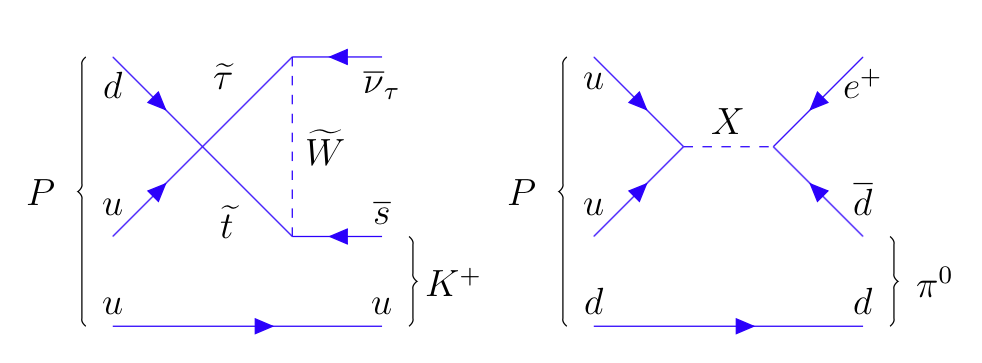
\includegraphics[width=6.5in]{Chapter-1/Images/MandatoryFeynmannDiagrams.png}
\caption{Feynman diagrams for proton decay ``golden modes": $p \rightarrow K^+ \bar{\nu}$ for supersymmetric GUTs on the left and  $p \rightarrow e^+ \pi^0$ for gauge-mediated GUTs  on the right.}
\label{fig:MandatoryFeynmannDiagrams}
\end{figure}


LArIAT tiny active volume makes it impossible for the experiment to place competitive limits on nucleon decay searches.  However,  LArIAT provides excellent data to characterize kaons in liquid argon for the ``LAr golden mode", $p \rightarrow K^+ \bar{\nu}$.  The result of these studies will affect future proton decay searches in LArTPCs.  Previous work has been done to assess the potential identification efficiency for different decay modes in a LArTPC \cite{Bueno2007}, but, as the time of this  writing, no study of kaon selection efficiency in LArTPCs has been performed on data. 
The K$^+$-Ar interaction cross section has never been measured before and can affect the possibility of detecting and measuring kaons when produced in a proton decay event. 
Kaon interactions with argon can distort the kaon energy spectrum as well as change the topology of single kaon events. In a LArTPC, non-interacting kaons appear as straight tracks with a high ionization depositions at the end (Bragg peak). The topology of interacting kaons can be quite different. In case of elastic scattering, a distinct kink will be present in the track. In case of inelastic scattering the Bragg peak will not be present and additional tracks will populate the event.
Performing the total hadronic K$^+$-Ar cross section measurement on data serves the double purpose of identifying the rate of ``unusual" topologies (kinks and additional tracks) and of developing tools for kaon tracking in LAr.

\subsubsection{K$^{+}$Ar Cross section in the Context of Light Mesons Interaction with Nuclei}
\label{sec:theoryStrangeMeson}
The intrinsic value of the total hadronic K$^{+}$-Ar cross section measurement is that kaon interactions complement the measurements of $\pi$ interactions as a probe of  hadron interaction inside the nucleus in the strange sector.  
\textcolor{red}{High theoretical interest in probing constituent quark model of nuclear structure with
KAON-NUCLEON INTERACTIONS CHIEDI REFERENZE A FLAVIO}


%Total cross sections for the interaction of mildly relativistic kaons with several nuclei were derived from transmission experiments performed at the alternating-gradient synchrotron in Brookhaven National Laboratory. The high precision of these cross sections ~about 1\% led to analyses of the data in terms of KN nucleus potentials, based on the expectation that the KN nucleus interaction is simply related to the KN interaction. In particular, in this energy range the KN interaction does not vary strongly with energy and together with the relative weakness of the interaction, one expects that optical potentials close to the ??tr?? approximation ~see below will be capable of describing the data. However, all such analyses showed disagreement between calculation and experiment at the level of 5?15\%, which caused speculations about modifications in the nuclear medium of the KN interaction @5?8#. 

\subsubsection{Signal Signatures}\label{sec:KSignalSignature}
%%%%%%%%%%%%%%%%%%%%%%%%%%%%%%%%%%%%%%%%%%%%%%%%%%%%%%%%%%%%%%%%%%%%%%%%%%%%%%%%%
The interaction of a mildly relativistic charged kaon with an argon nucleus is determined largely by the strong force. The total hadronic K$^{+}$-Ar interaction cross section is defined as the one related to the single (hadronic) process driven only by the strong interaction.
In this case, ``total" indicates all strong interactions regardless of the final state. This condition purposefully includes both elastic and inelastic (reaction) channels. Indeed, the total cross section section can be then decomposed into
$$\sigma_{Tot} = \sigma_{Elastic}+ \sigma_{Reaction}.$$


%For this analysis, kaons are selected from the LArIAT beamline in the momentum range between \textcolor{red}{500} MeV/c and \textcolor{red}{1000} MeV/c (see Fig \ref{fig:TOFK}).

%\begin{figure}[hpbt]
%\centering
%\includegraphics[width=5in]{Chapter-1/Images/KaonTOF}
%\caption{Time of flight versus momentum distributions as produced by the LArIAT TOF and Wire Chambers systems. The Kaon population lies between the proton and the muon/pion populations, allowing PID of Kaons in the beam line.  }
%\label{fig:TOFK}
%\end{figure}

For the LArIAT cross section analysis, the kaons considered span a momentum inside the TPC from 800 MeV/c and 100 MeV/c. In this energy range, the relevant K-Nucleon interactions are according to \cite{fesbach1992theoretical}:

\begin{align}
K^{+} + N &\rightarrow K^{+} + N\textit{ (elastic)}\\
K^{+} + n &\rightarrow K^{0} + p\textit{ (elastic)}\\
K^{+} + N &\rightarrow K + N + \pi \textit{ (inelastic)}\\
K^{+} + N &\rightarrow K^{*} + N\textit{ (inelastic)}.
\end{align}

\subsubsection{Previous Measurements: Lighter and Heavier Nuclei}
In general, measurements on kaon cross sections are  extremely scarce. The measurement of the kaon interaction cross section would bring the additional benefit of reducing the uncertainties associated  with hadron interaction models adopted in MC simulations for argon targets, beneficial for both proton decay studies and kaon production from neutrino interaction studies, where the  uncertainties for final state interaction models are big \cite{Drakoulakos:2004gn}. 

Figure \ref{fig:Friedmann} shows a 1997 measurement on several elements as performed by  Friedmann et al.  \cite{Friedman:1997eq}. As a reference, this paper measures a $\sigma_{Tot}$ for Si of  366.5  $\pm$  4.8 mb and a $\sigma_{Tot}$ for Ca of 494.6  $\pm$ 7.7 mb at 488 MeV/c.  The cross section for argon is expected to lie in between these two measurements. 
Additional data on the kaon cross section are provided by Bugg et al. \cite{PhysRev.168.1466}. Bugg performs a measurement of the total 
K$^+$ and K$^-$ cross sections on protons and deuterons over the range of 0.6-2.65 GeV/c, as well as a measurement of the total K$^+$ and K$^-$  cross sections on carbon for a number of momenta; the results of this paper on carbon are reported in Figure \ref{fig:Bugg}.



\begin{figure}
\captionsetup{justification=raggedright}  
	\begin{minipage}[t]{.53\textwidth}  
	  \centering  
	   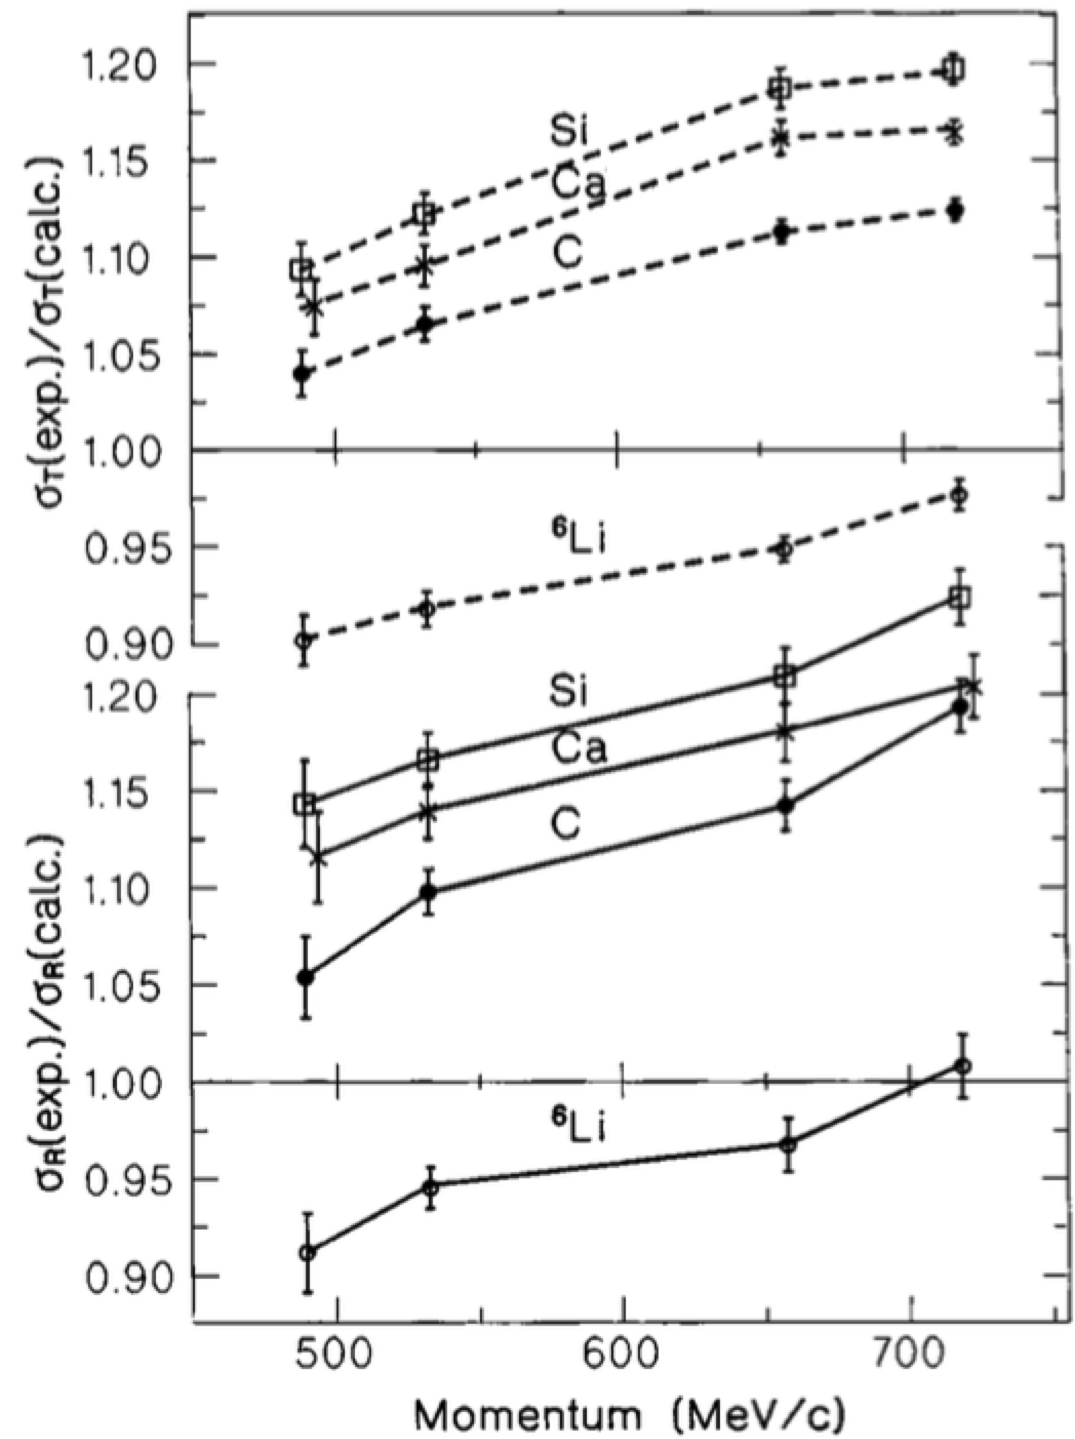
\includegraphics[width=3in]{Chapter-1/Images/Friedmann.png}
	   	        \caption{Ratios between experimental and calculated cross sections as from \cite{Friedman:1997eq}. Top: Total cross sections. \\Bottom: reaction cross sections.}
        \label{fig:Friedmann}
	\end{minipage}%  
	\begin{minipage}[t]{0.53\textwidth}  
	  \centering  
	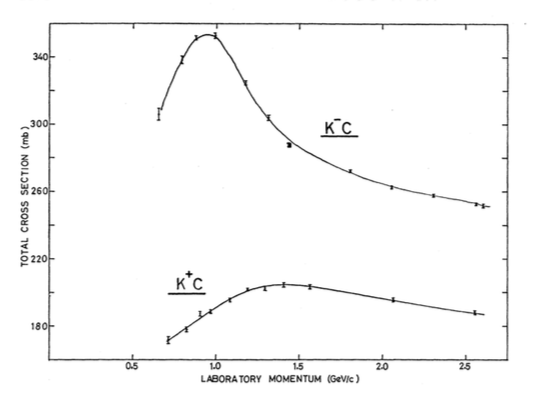
\includegraphics[width=3in]{Chapter-1/Images/Bugg.png}
        \caption{Total K$^+$  and K$^-$ cross sections on carbon as from \cite{PhysRev.168.1466}.}
        \label{fig:Bugg}
	\end{minipage}
	\par
\end{figure}



%%%%%%%%%%%%%%%%%%%%%%%%%%%%%%%%%%%%%%%%%%%%%%%%%%%%%%%
%% PRETTY EVENT DISPLAY WITH TEXT, NOT SURE IF USEFUL
%\begin{figure}[h!]
%\centering
%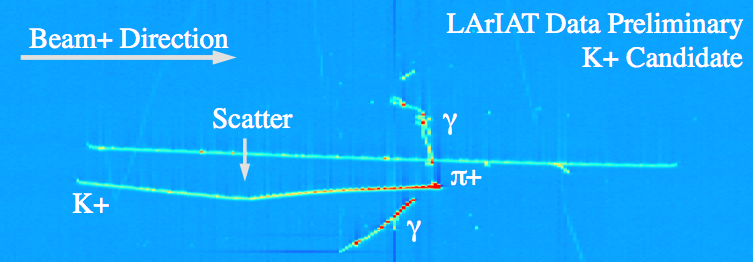
\includegraphics[width=6.5in]{Chapter-1/Images/KLariat.png}
%\caption{LArIAT Data $K^+$ candidate. $K^+$ enters TPC, undergoes a hadronic scatter, and then decays into $\pi^+$ and $\pi^0$. The the $\pi^0$ decays into 2 photons while the $\pi^+$ stops quickly in the TPC. Collection plane view.}
%\label{Fig:KLariat}
%\end{figure}

%Fig \ref{Fig:KLariat} shows a $K^+$ candidate event in the LArIAT TPC. Following the kaon candidate track from left to right, two important elements are visible by eye: a change in the K momentum due to hadronic scatter and a Bragg peak by the end of the track due to an augment of ionization as the kaon slows down in the TPC. The track "kink" is only visible thanks to the millimetric spacial resolution of the TPC, while the Bragg shows the calorimetric power of this technology. The kaon in this event decays hadronically into $\pi^+$ and $\pi^0$. The the $\pi^0$ decays into 2 photons while the $\pi^+$ stops quickly in the TPC. The ability to distinguish the topology of this decay from the most frequent one, i.e. $K^+\rightarrow\mu^+\nu$, remarks the versatility of the LArTPC technology.
%%%%%%%%%%%%%%%%%%%%%%%%%%%%%%%%%%%%%%%%%%%%%%%%%%%%%%%




 \subsubsection{Kaon Interaction Cross Section for thin target in Geant4}
Since the kaon cross section in argon has never been measured before, simulation packages tune kaon transportation in argon by extrapolation from lighter and heavier nuclei. LArIAT uses the Geant4 suite for particle transportation.  Since kaon data on carbon are available, we used it as a metric to evaluate the Geant4 prediction performances.  Figure \ref{fig:TrueCarbon} shows the total hadronic cross section for carbon implemented in Geant4 10.01.p3 overlaid with the Bugg and Friedman data. Unfortunately, the current version of Geant4 does not reproduce the data for carbon closely. On one hand, this evidence makes us even more wary when using the Monte Carlo in simulating the kaon-argon interactions. On the other, it further highlights the importance of the kaon measurement.



\begin{figure}
\captionsetup{justification=raggedright}  
  \centering  
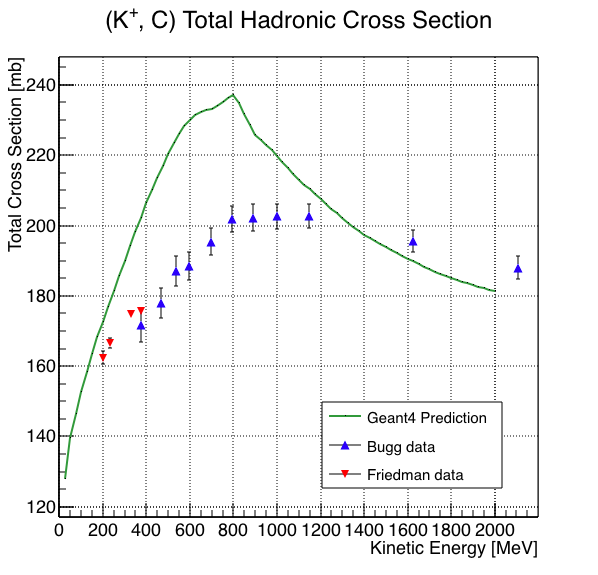
\includegraphics[width=3in]{Chapter-1/Images/CarbonG4.png}
\caption{total hadronic cross section for carbon implemented in Geant4  10.01.p3  with overlaid with the Bugg and Frideman data.}
\label{fig:TrueCarbon}
\end{figure}






